\section{Modelo Relacional}

En esta etapa se procede con la conversión del Modelo Entidad-Relación (MER) al Modelo Relacional (MR). El MER de referencia, en el que se ha resuelto la especialización/generalización, se muestra en la Figura \ref{f:mersh}. La siguiente descripción se enfocará exclusivamente en las tablas generadas a partir de relaciones complejas (N:M, ternarias) o aquellas que requirieron modificaciones estructurales. Las entidades que no se detallen a continuación se mapean a tablas de forma directa, conservando su estructura original.
\subsection{Conversión Relaciones N-arias}\label{s:mr1}



\subsubsection{Supervisar}
Al transformar el Modelo Entidad-Relación (MER) al Modelo Relacional (MR), la relación ternaria \texttt{Supervisar} (Figura \ref{f:mersupervisar2}) se convierte en una nueva tabla. Esta tabla, también llamada \texttt{Supervisar}, incluye las claves foráneas de las tres entidades participantes: \texttt{Proyecto}, \texttt{Alumno} y \texttt{Profesor}.

La clave primaria para esta nueva tabla se define a partir de la dependencia funcional del requisito \ref{linea9}: como un par (\texttt{Alumno}, \texttt{Proyecto}) determina a un único \texttt{Profesor} supervisor, la clave primaria de la tabla \texttt{Supervisar} se compone únicamente de las claves foráneas de \texttt{Alumno} y \texttt{Proyecto}. La clave del \texttt{Profesor}, al ser determinada por las otras dos, se mantiene como un atributo no clave. La estructura resultante se detalla en la Tabla \ref{tab:mrsupervisar}.

\begin{figure}[H]
\centering
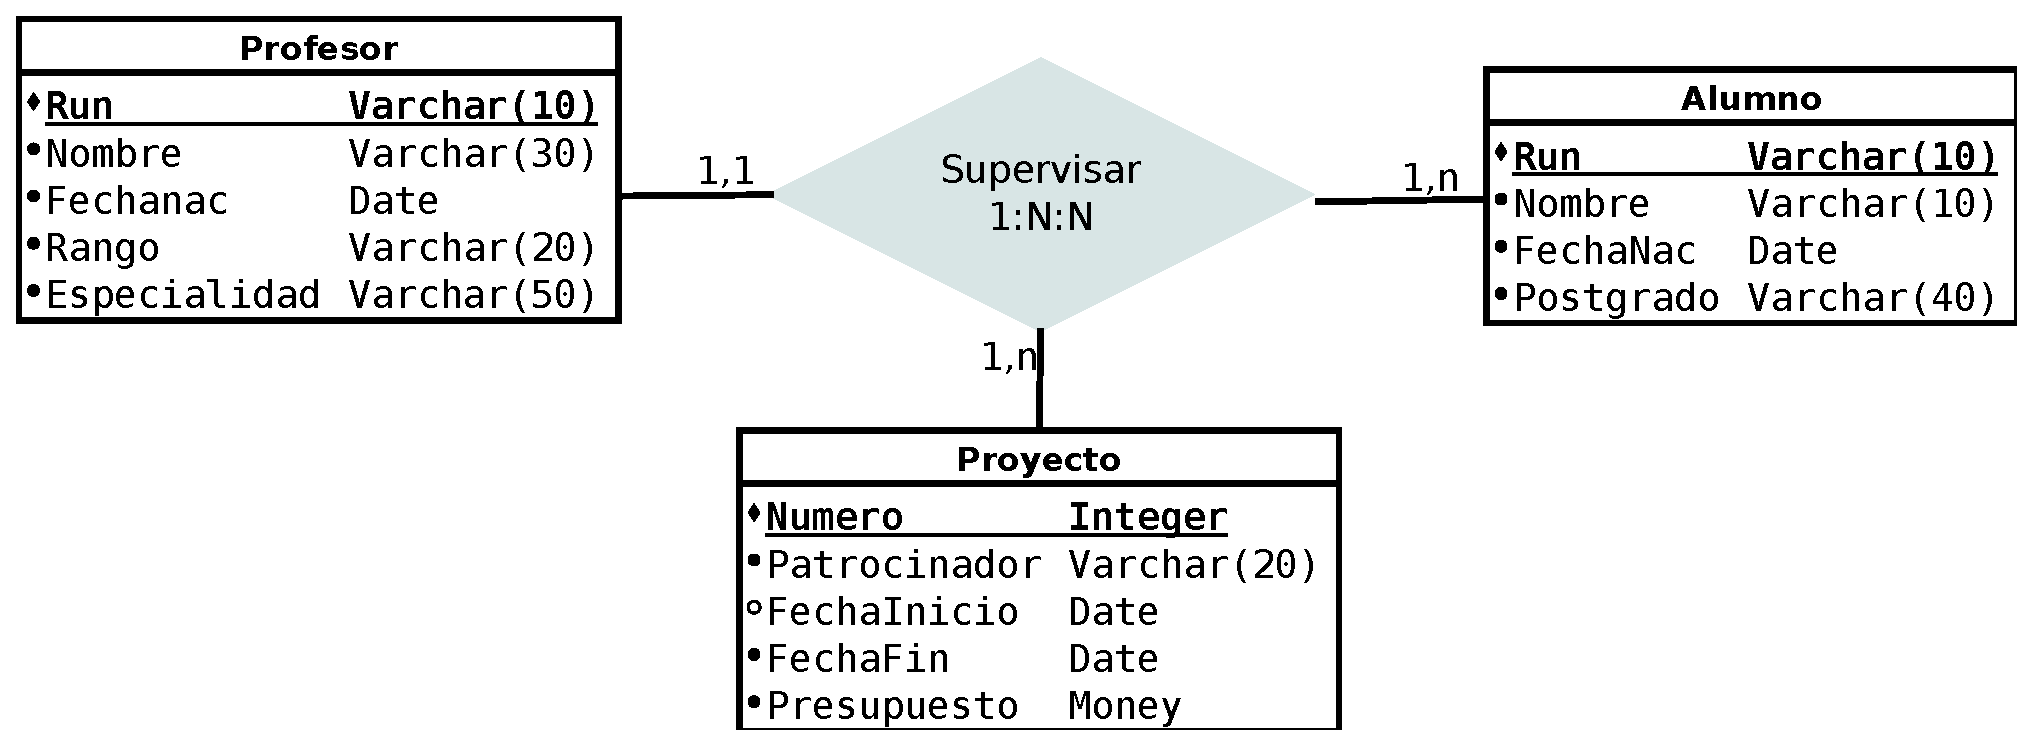
\includegraphics[width=0.8\textwidth]{images/MR/supervisar_nan.eps}
    \caption{Relación Supervisar}
    \label{f:mersupervisar2}
\end{figure}


\begin{table}[H]
    \centering
    \begin{tabular}{|ll|}\hline
    \multicolumn{2}{|c|}{\textbf{Supervisar}}\\\hline
         \textbf{Proyecto\_id} (PFK)&Integer \\
       \textbf{Alumno\_id} (PFK) & Varchar(10)\\
       \textbf{Profesor\_id} (FK) & Varchar(10)\\\hline
    \end{tabular}
    \caption{MR de la Relación Supervisar}
    \label{tab:mrsupervisar}
\end{table}

\subsection{Conversión Relaciones N:N}\label{s:mr2}
\subsubsection{Dirigir}
En el proceso de conversión del Modelo Entidad-Relación (MER) al Modelo Relacional (MR), la relación de muchos a muchos (N:M) \texttt{Dirigir}, ilustrada en la Figura \ref{f:merdirigir2}, se transforma en una nueva tabla. Esta tabla, también denominada \texttt{Dirigir}, hereda como claves foráneas las claves primarias de las entidades que relaciona (\texttt{Proyecto} y \texttt{Profesor}), y la combinación de ambas conforma su nueva clave primaria. La estructura final se presenta en la Tabla \ref{tab:mrdirigir}.

\begin{figure}[H]
\centering
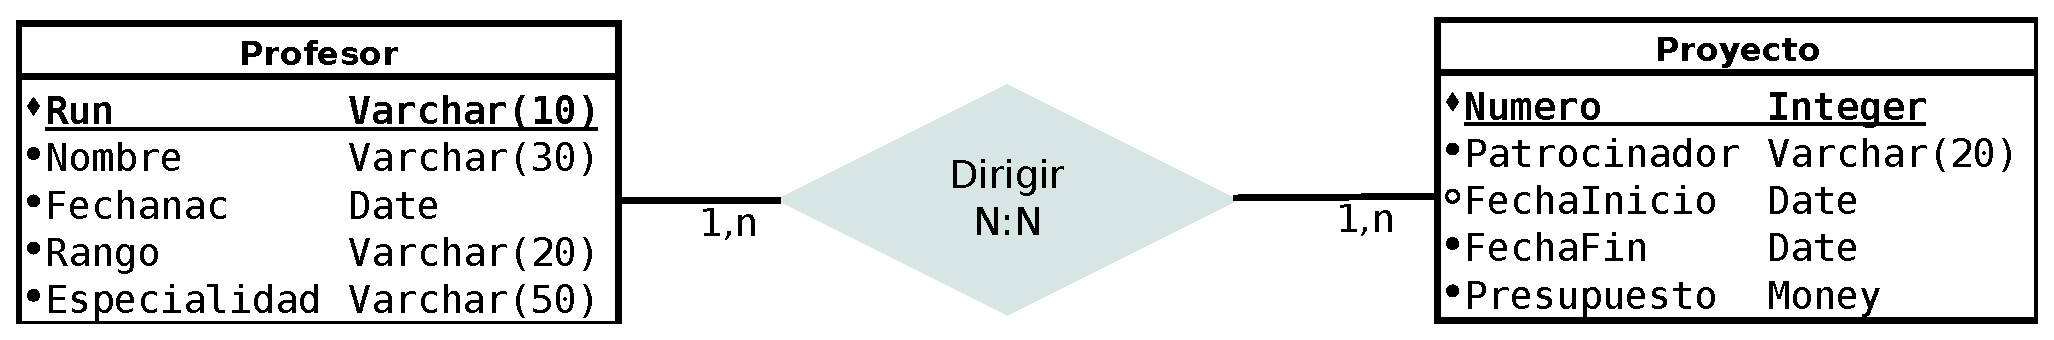
\includegraphics[width=0.8\textwidth]{images/MR/dirigir_nan.eps}
    \caption{Relación Dirigir}
    \label{f:merdirigir2}
\end{figure}

\begin{table}[H]
    \centering
    \begin{tabular}{|ll|}\hline
    \multicolumn{2}{|c|}{\textbf{Dirigir}}\\\hline
         \textbf{Proyecto\_id} (PFK)&Integer \\
       \textbf{Profesor\_id} (PFK) & Varchar(10)\\\hline
    \end{tabular}
    \caption{MR de la Relación Dirigir}
    \label{tab:mrdirigir}
\end{table}

\subsubsection{Laborar}
En el proceso de conversión del MER al Modelo Relacional, la relación N:M \texttt{Laborar} (Figura \ref{f:merlaborar2}) da origen a una nueva tabla. Dicha tabla, llamada \texttt{Laborar}, hereda las claves primarias de \texttt{Profesor} y \texttt{Departamento} para formar su propia clave primaria compuesta. Adicionalmente, se incluye como atributo no clave el \texttt{Porcentaje} que pertenecía a la relación. La estructura resultante se detalla en la Tabla \ref{tab:mrlaborar}.

\begin{figure}[H]
\centering
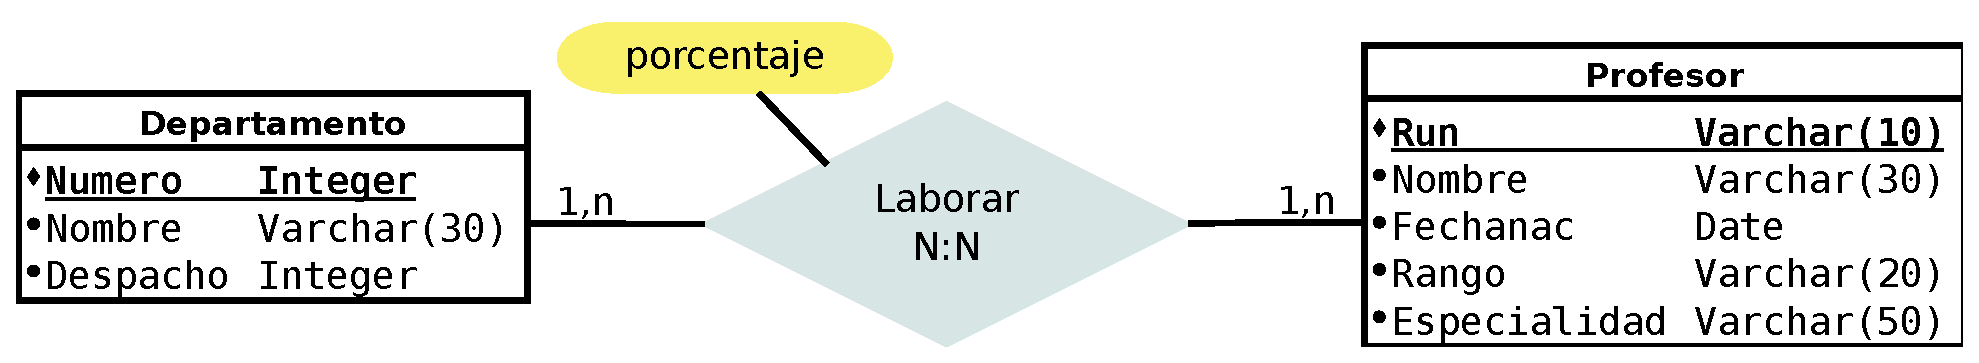
\includegraphics[width=0.8\textwidth]{images/MR/laborar_nan.eps}
    \caption{Relación Laborar}
    \label{f:merlaborar2}
\end{figure}

\begin{table}[H]
    \centering
    \begin{tabular}{|ll|}\hline
    \multicolumn{2}{|c|}{\textbf{Laborar}}\\\hline
         \textbf{Departameno\_id} (PFK)&Integer \\
       \textbf{Profesor\_id} (PFK) & Varchar(10)\\
       Porcentaje&Integer\\\hline
    \end{tabular}
    \caption{MR de la Relación Laborar}
    \label{tab:mrlaborar}
\end{table}

\subsubsection{Trabajar}

La relación \texttt{Trabajar}, representada en la Figura \ref{f:mertrabajar2}, es una relación de cardinalidad muchos a muchos (N:M) entre \texttt{Proyecto} y \texttt{Alumno}. Durante el proceso de conversión del Modelo Entidad-Relación (MER) al Modelo Relacional (MR), este tipo de relación se transforma en una nueva tabla. Para este caso, dicha transformación da origen a la tabla \texttt{Trabajar}, presentada en la Tabla \ref{tab:mrtrabajar}.

\begin{figure}[H]
\centering
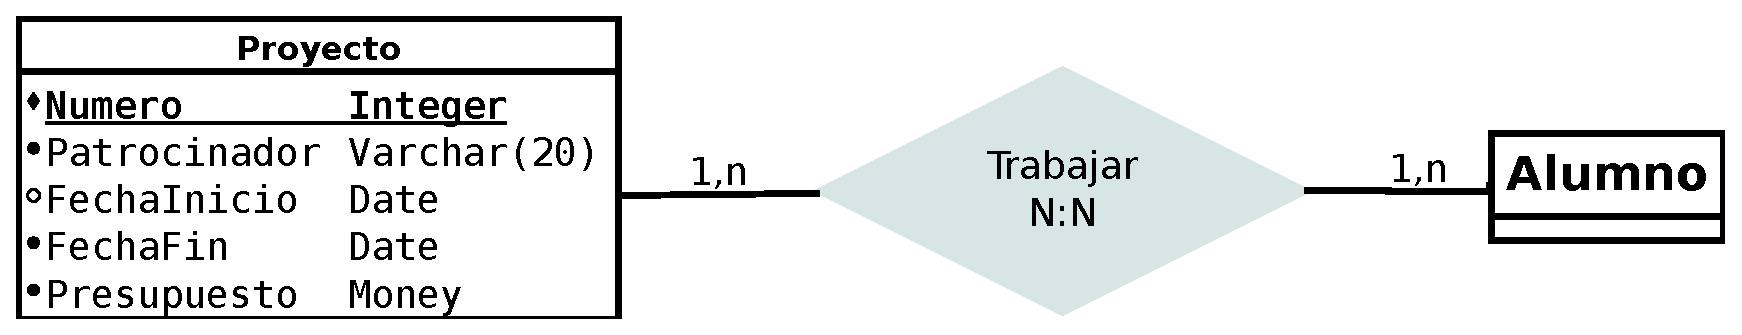
\includegraphics[width=0.8\textwidth]{images/MR/trabajar_nan.eps}
    \caption{Relación Trabajar}
    \label{f:mertrabajar2}
\end{figure}

\begin{table}[H]
    \centering
    \begin{tabular}{|ll|}\hline
    \multicolumn{2}{|c|}{\textbf{Trabajar}}\\\hline
         \textbf{Proyecto\_id} (PFK)&Integer \\
       \textbf{Alumno\_id} (PFK) & Varchar(10)\\\hline
    \end{tabular}
    \caption{MR de la Relación Trabajar}
    \label{tab:mrtrabajar}
\end{table}

\subsection{Conversión Relaciones 1:N}\label{s:mr3}
\subsubsection{Cursar}
Al transformar el Modelo Entidad-Relación (MER) al Modelo Relacional (MR), la relación de uno a muchos (1:N) \texttt{Cursar} (Figura \ref{f:mercursar2}) se resuelve siguiendo la regla estándar para este tipo de cardinalidad, la cual no requiere la creación de una tabla nueva para la relación.

El procedimiento correcto consiste en propagar la clave primaria de la entidad del lado ``1'' de la relación (\texttt{Postgrado}) a la tabla de la entidad del lado ``N'' (\texttt{Alumno}). Específicamente:
\begin{itemize}
\item Se añade una columna de clave foránea en la tabla \texttt{Alumno} que haga referencia a la clave primaria de \texttt{Postgrado}.
\item Dado que el requisito de la línea \ref{linea4} indica que la participación del alumno es opcional (`puede o no pertenecer'), esta nueva columna de clave foránea en la tabla \texttt{Alumno} debe permitir valores \texttt{NULL}.
\end{itemize}
Este enfoque es más eficiente y evita la creación de una tabla adicional innecesaria. La Tabla \ref{tab:mrcursar}  muestra la estructura de la tabla \texttt{Alumno} modificada para incluir esta clave foránea.
\begin{figure}[H]
\centering
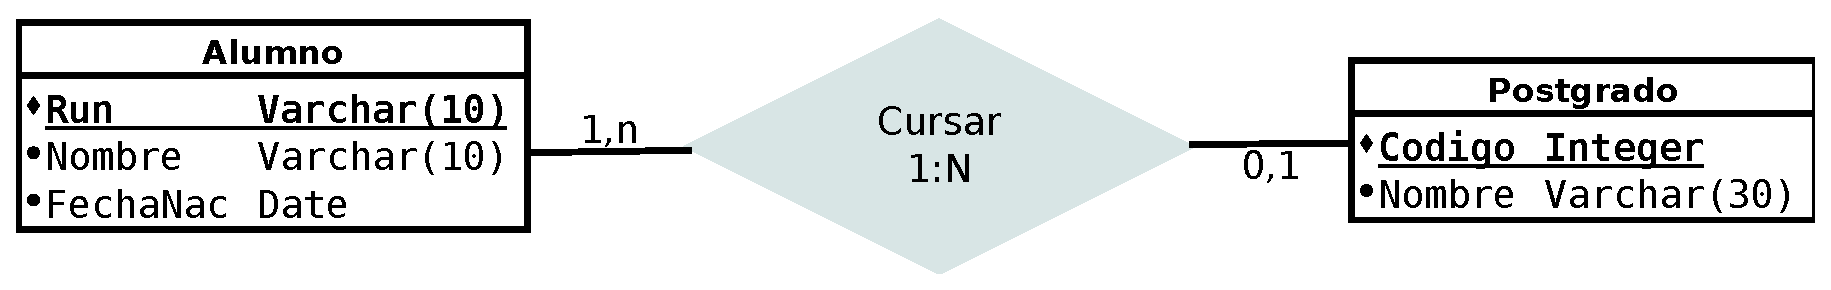
\includegraphics[width=0.8\textwidth]{images/MR/cursar_1an.eps}
    \caption{Relación Cursar}
    \label{f:mercursar2}
\end{figure}

\begin{table}[H]
    \centering
    \begin{tabular}{|ll|}\hline
    \multicolumn{2}{|c|}{\textbf{Alumno}}\\\hline
         \textbf{Run} (PK)&Varchar(10) \\
       Nombre & Varchar(40)\\
       Fechanac&Date\\
       \textit{Postgrado\_id} (FK)& Integer\\
       \hline
    \end{tabular}
    \caption{MR de la Relación Cursar}
    \label{tab:mrcursar}
\end{table}

\subsubsection{Pertenece}

Al transformar la relación de uno a muchos (1:N) \texttt{Pertenece} (Figura \ref{f:merpertencer2}) al Modelo Relacional, se aplica la regla de propagación de claves. El procedimiento es el siguiente:
\begin{itemize}
\item La clave primaria de la entidad en el lado ``uno'' de la relación (\texttt{Departamento}) se propaga a la tabla de la entidad en el lado ``muchos'' (\texttt{Alumno}).
\item La clave primaria de \texttt{Departamento} (\texttt{Numero}), se añade como clave foránea a la tabla \texttt{A\-lum\-no}.
\item Como la participación del \texttt{Alumno} es obligatoria (1,1), según se infiere de la línea \ref{linea13}, estas nuevas columnas en la tabla \texttt{Alumno} no deben permitir valores nulos.
\end{itemize}
La estructura resultante de la tabla \texttt{Alumno} se detalla en la Tabla \ref{tab:mrpertencer}.



\begin{figure}[H]
\centering
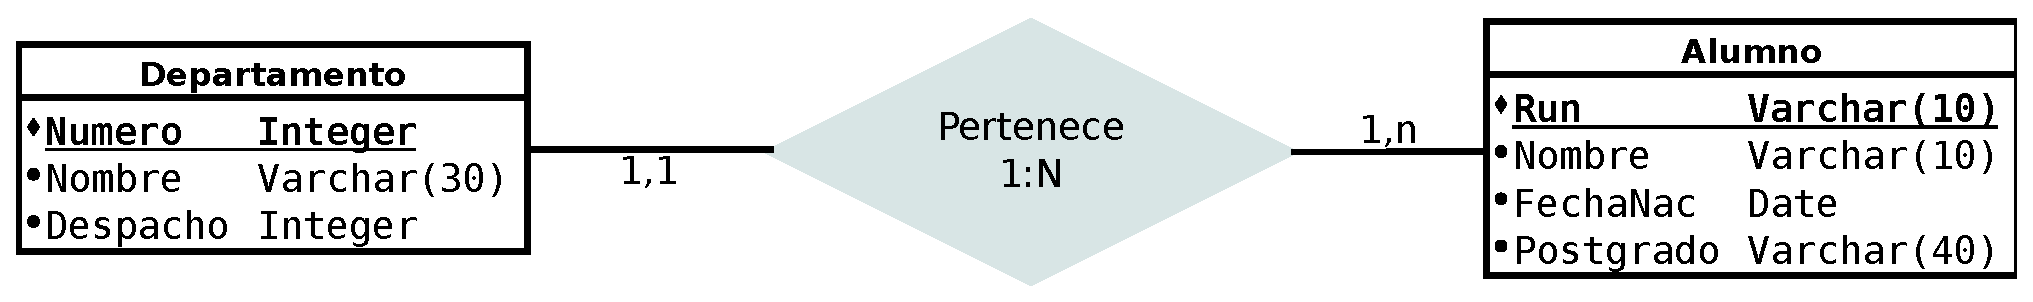
\includegraphics[width=0.8\textwidth]{images/MR/pertenece_1an.eps}
    \caption{Relación Pertenece}
    \label{f:merpertencer2}
\end{figure}


\begin{table}[H]
    \centering
    \begin{tabular}{|ll|}\hline
    \multicolumn{2}{|c|}{\textbf{Alumno}}\\\hline
         \textbf{Run} (PK)&Varchar(10) \\
       Nombre & Varchar(40)\\
       Fechanac&Date\\
              \textit{Postgrado\_id} (FK)& Integer\\
       \textit{Departamento\_id} (FK)&Integer\\
       \hline
    \end{tabular}
    \caption{MR de la Relación Pertenece}
    \label{tab:mrpertencer}
\end{table}

\subsection{Conversión Relaciones 1:1}\label{s:mr4}
\subsubsection{Administrar}

Para convertir la relación de uno a uno (1:1) \texttt{Administrar} (Figura \ref{f:meradministrar2}) al Modelo Relacional, se utiliza el método de propagación de claves. La dirección de esta propagación se decide en función de la participación de cada entidad. Se propaga la clave primaria de la entidad con participación opcional a la tabla de la entidad con participación obligatoria.
\begin{itemize}
    \item La entidad \texttt{Departamento} tiene participación obligatoria y única (1,1).
\item La entidad \texttt{Profesor} tiene participación opcional y única (0,1).
\end{itemize}

Para optimizar el diseño, la clave primaria de \texttt{Profesor} se añade como clave foránea en la tabla \texttt{Departamento}. Para garantizar la integridad de la relación 1:1, esta nueva columna debe ser \texttt{NOT NULL} y \texttt{UNIQUE}. La estructura resultante se detalla en la Tabla \ref{tab:mradministrar}.




\begin{figure}[H]
\centering
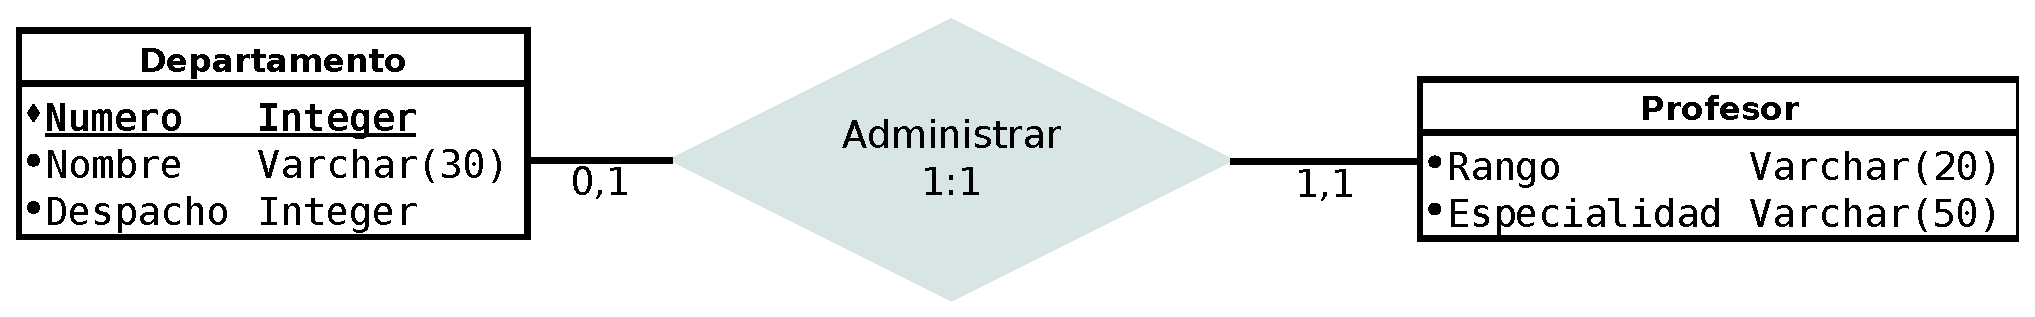
\includegraphics[width=0.8\textwidth]{images/MR/administrar_1a1.eps}
    \caption{Relación Administrar}
    \label{f:meradministrar2}
\end{figure}


\begin{table}[H]
    \centering
    \begin{tabular}{|ll|}\hline
    \multicolumn{2}{|c|}{\textbf{Departamento}}\\\hline
    \textbf{Numero} (PK)& Integer\\
    Nombre &Varchar(30)\\
    Despacho&Integer\\
    \textit{Profesor\_id} (FUK)&Varchar(10) \\
       \hline
    \end{tabular}
    \caption{MR de la Relación Administrar}
    \label{tab:mradministrar}
\end{table}


\subsection{Conversión Relaciones Reflexivas y otras}\label{s:mr5}
\subsubsection{Asesorar}

 A partir del requisito de la línea \ref{linea14}, se define la relación reflexiva (o recursiva) \texttt{Asesorar} sobre la propia entidad \texttt{Alumno}. Como se ilustra en la Figura \ref{f:merasesorar2}, esta es una relación de uno a muchos (1:N) que distingue los roles de ``asesor'' y ``asesorado'':
\begin{itemize}
    \item Un \texttt{Alumno} (en el rol de asesor) puede asesorar a uno o muchos otros alumnos (1,N).
\item Cada \texttt{Alumno} (en el rol de asesorado) debe tener exactamente un asesor (1,1).
\end{itemize}

Para implementar esto en el Modelo Relacional, se añade una clave foránea en la tabla \texttt{Alumno} que se referencia a sí misma, como se muestra en la Tabla \ref{tab:mrasesorar}.


\begin{figure}[H]
\centering
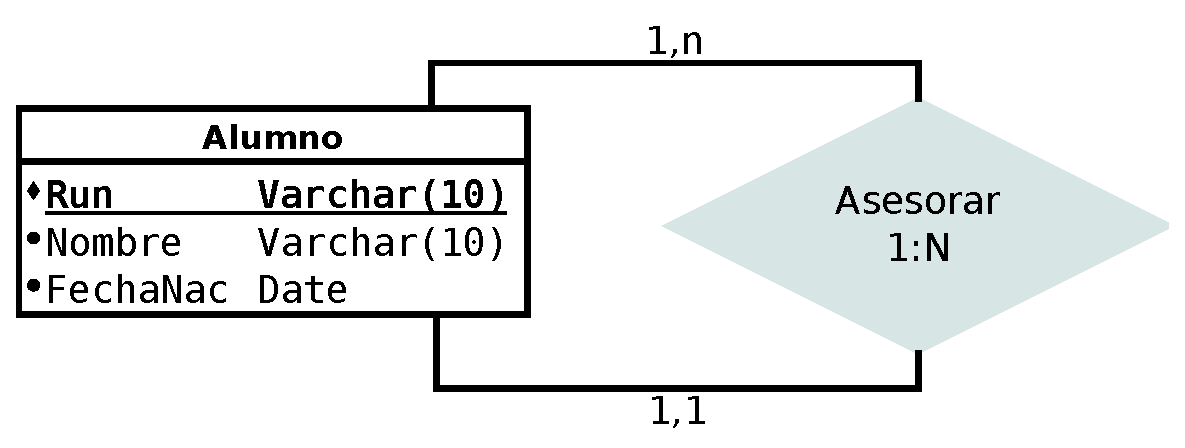
\includegraphics[width=0.6\textwidth]{images/MR/asesorar_1an.eps}
    \caption{Relación Asesorar}
    \label{f:merasesorar2}
\end{figure}

\begin{table}[H]
    \centering
    \begin{tabular}{|ll|}\hline
    \multicolumn{2}{|c|}{\textbf{Alumno}}\\\hline
         \textbf{Run} (PK)&Varchar(10) \\
       Nombre & Varchar(40)\\
       Fechanac&Date\\
                     \textit{Postgrado\_id} (FK)& Integer\\
       \textit{Departamento\_id} (FK)&Integer\\
       \textit{Alumno\_id} (FK)&Varchar(10)\\
       \hline
    \end{tabular}
    \caption{MR de la Relación Asesorar}
    \label{tab:mrasesorar}
\end{table}





\begin{landscape}
\subsection{Modelo Relacional Resultante}
Una vez realizadas las conversiones presentadas en las secciones \ref{s:mr1}-\ref{s:mr5} se obtienen las entidades que se ven en la Figura \ref{f:mr}.
\begin{figure}[H]
    \centering
 \includegraphics[width=1\linewidth]{images/MR/MR_Universidad_Casoestudio.png}
        \caption{Modelo Relacional de la universidad}
    \label{f:mr}
\end{figure}
\end{landscape}
